% 
\chapter{Implementação da Solução} 
\label{chap:Impl} % For referencing the chapter elsewhere, use Chapter~\ref{Impl}

Neste capítulo, será apresentada a implementação da solução com recurso a alguns exemplos de desenvolvimento, interfaces de utilizador e a integração com serviços da \gls{AWS}.

Poderá ser confirmada o uso da arquitetura modelada no capítulo~\ref{chap:ADS}, e de que forma os casos de uso e os requisitos funcionais foram implementados.

Nesta secção, são mostrados testes tanto de domínio, como testes \textit{end-2-end}.

%-------------------------------------------------------------------------------

\section{Descrição da implementação} 
\label{sec:desc} %For referencing this section elsewhere, use Section~\ref{sec:desc}

Nesta secção, estão evidenciadas decisões, tecnologias e a forma como diferentes componentes da solução foram concretizados, assegurando a coerência com a arquitetura e a solução. 

Para esta descrição, apresentou-se partes da solução e foram utilizados dados de teste, que não contemplam quaisquer informações reais.

\subsection{\textbf{Low Latency Chat}}

A solução descreve uma arquitetura em tempo real entre utilizadores ligados a uma mesma transmissão, garantindo o registo das ligações, difusão eficiente de mensagens e a eliminação dessa conecção após a saida da transmissão. Para tal efeito, foram usados alguns serviços AWS:

\begin{itemize}
    \item API Gateway WebSocket
    \item AWS Lambda
    \item Amazon DynamoDB
\end{itemize}

A \textit{web-socket} é composta por três rotas \textbf{\$connect}, \textbf{\$disconect} e \textbf{\$sendChatMessage}, e cada uma dessas rotas quando alcançada pelo utilizador promove uma chamada às funções \textit{serverless} (Lambda).

Segue-se o codigo das funções Lambda:

\begin{lstlisting}[language=Java, caption={Ligação ao Chat}, label={lst:ChatConnect}]
    const { DynamoDBClient, PutItemCommand } = require("@aws-sdk/client-dynamodb");
const client = new DynamoDBClient({ region: "eu-west-1" });

exports.handler = async (event) => {
  console.log("event", event);
  const streamId = event.queryStringParameters?.streamId || "default";
  console.log("streamId", streamId);
  const connectionId = event.requestContext.connectionId;
  console.log("connectionId", connectionId);

  const command = new PutItemCommand({
    TableName: "liveChat",
    Item: {
      streamId: { S: streamId },
      connectionId: { S: connectionId },
      timestamp: { N: `${Date.now()}` }
    }
  });

  await client.send(command);
  return { statusCode: 200 };
};
\end{lstlisting}

Nesta função~\ref{lst:ChatConnect} o utilizador entra na página da transmissão que tem um \textit{streamId} associado, e um \textit{connectionId} fornecido pela API Gateway. Após a entrada o registo do utilizador é guardado na tabela \textit{liveChat}.

\begin{lstlisting}[language=Java, caption={Remoção do Chat}, label={lst:ChatDisconect}]
const { DynamoDBClient, DeleteItemCommand, ScanCommand } = require("@aws-sdk/client-dynamodb");
const client = new DynamoDBClient({ region: "eu-west-1" });

exports.handler = async (event) => {
  const connectionId = event.requestContext.connectionId;
  const scan = new ScanCommand({
    TableName: "liveChat",
    FilterExpression: "connectionId = :conn",
    ExpressionAttributeValues: {
      ":conn": { S: connectionId }
    }
  });

  const result = await client.send(scan);
  const item = result.Items?.[0];
  if (!item) return { statusCode: 200 };

  const streamId = item.streamId.S;
  console.log("streamId", streamId);
  const del = new DeleteItemCommand({
    TableName: "liveChat",
    Key: {
      streamId: { S: streamId },
      connectionId: { S: connectionId }
    }
  });

  await client.send(del);
  return { statusCode: 200 };
};    
\end{lstlisting}

Nesta função~\ref{lst:ChatDisconect} a remoção do registo do utilizador é feita independentemente se ele sai da sala de transmissão diretamente, ou, se fecha o \textit{browser}. Assim a base de dados não fica com registo errados.

\begin{lstlisting}[language=Java, caption={Envio das Mensagens}, label={lst:chatsendMessage}]
exports.handler = async (event) => {
  let streamId, message;
  try {
    const body = typeof event.body === 'string' ? JSON.parse(event.body) : event.body;
    streamId = body.streamId;
    message = body.message;
  } catch (err) {
    console.error('Erro a fazer parse ao body:', event.body);
    return { statusCode: 400, body: 'Invalid JSON body' };
  }
  try {
    const connections = await ddb.query({
      TableName: 'liveChat',
      KeyConditionExpression: 'streamId = :s',
      ExpressionAttributeValues: {
        ':s': streamId
      },
    }).promise();

    // 2. Enviar a mensagem para cada connectionId
    const postCalls = connections.Items.map(async ({ connectionId }) => {
      try {
        await apigw.postToConnection({
          ConnectionId: connectionId,
          Data: JSON.stringify({ message }),
        }).promise();
      } catch (err) {
        if (err.statusCode === 410) {
          console.log(`Stale connection: ${connectionId}`);
        } else {
          console.error(`Failed to send to ${connectionId}:`, err);
        }
      }
    });

    await Promise.all(postCalls);

    return { statusCode: 200, body: 'Message sent.' };
  } catch (err) {
    console.error('Error broadcasting message:', err);
    return { statusCode: 500, body: 'Internal error' };
  }
};   
\end{lstlisting}

Na função~\ref{lst:chatsendMessage}, dão entrada o \textit{streamId} e a mensagem, é consultada a tabela \textit{liveChat} onde são retirados os \textit{id's} dos utilizadores presentes na transmissão, e procede-se ao envio das mensagens para cada ligação através da \textit{web-socket}.

A imagem~\ref{fig-chat} mostram a interação de dois utilizadores:

\begin{figure}[H]
\centering
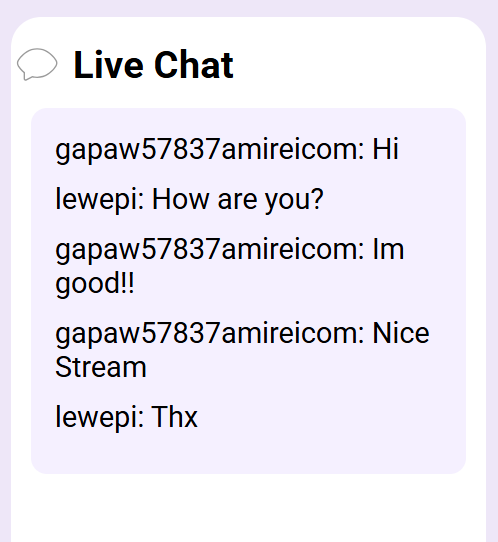
\includegraphics[width=\textwidth,height=0.2\textheight,keepaspectratio]{frontmatter/assets/Implementacao/chat.png}
\caption{Componente do \textit{low latency chat}}
\label{fig-chat}
\end{figure}

\subsection{\textbf{Tiers}}

Para o criador conseguir ter uma transmissão ao vivo, antes tem de definir níveis de acesso que permita algum utilizador entrar na sua página. Na figura~\ref{fig-escalao}

\begin{figure}[H]
\centering
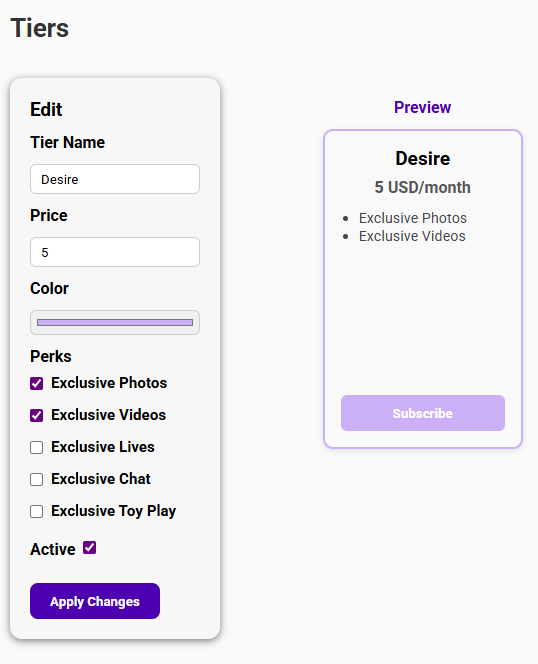
\includegraphics[width=\textwidth,height=0.4\textheight,keepaspectratio]{frontmatter/assets/Implementacao/tierAndPreview.png}
\caption{Edição e \textit{Preview} de um escalão de acesso}
\label{fig-escalao}
\end{figure}

Ao introduzir os dados necessários para criar um escalão: (\textit{Tier Name}, \textit{Tier Price}, \textit{Color}, e \textit{Perks}, o criador pode aplicar as mudanças/criar um escalão, e desde que tenha um nível com o benefício \textbf{Exclusive Lives}, consegue iniciar transmissão.

Do lado do utilizador normal, ao entrar no perfil privado do criador, depara-se com este menu ~\ref{fig-concent}:

\begin{figure}[H]
\centering
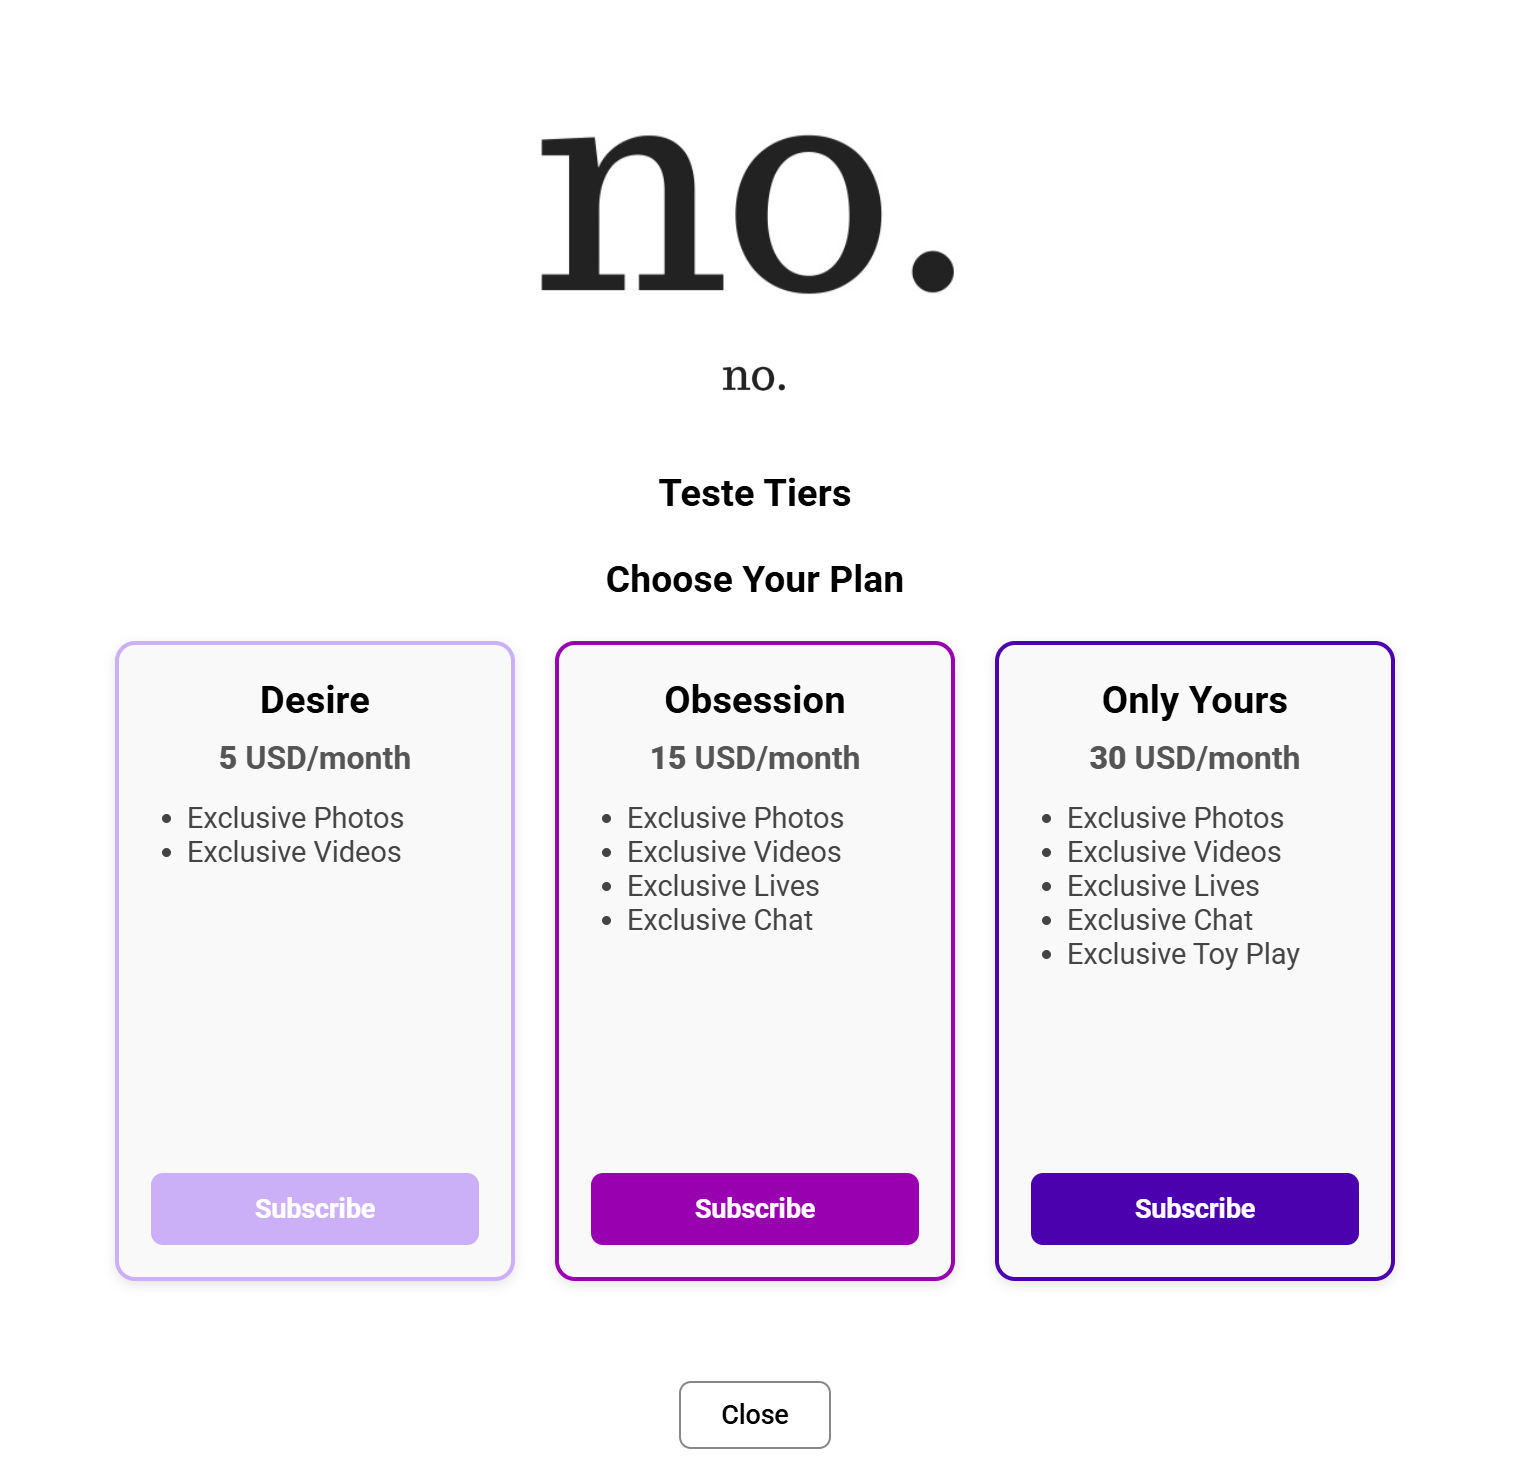
\includegraphics[width=\textwidth,height=0.4\textheight,keepaspectratio]{frontmatter/assets/Implementacao/consentimento.png}
\caption{Área de seleção de um escalão}
\label{fig-concent}
\end{figure}

Nesta área o visiualizador, consegue ver a foto de perfil bem como a capa do criador de conteúdo. 


\subsection{\textbf{Livestream Menu}}

Para tornar a transmissão mais mais interativa para o utilizador, o criador pode criar um menu com diversãs opções para fazer durante a transmissão. O menu é completamente editável, pode ter quinze opções com diferentes descrições e durante a transmissão o criador pode esconder essas opções.


\begin{figure}[H]
\centering
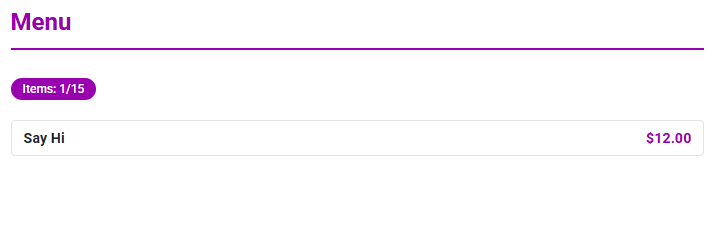
\includegraphics[width=\textwidth,height=0.2\textheight,keepaspectratio]{frontmatter/assets/Implementacao/menufromViewer.png}
\caption{Menu de \textit{Items} - Visualizador}
\label{fig-menuViewer}
\end{figure}

\begin{figure}[H]
\centering
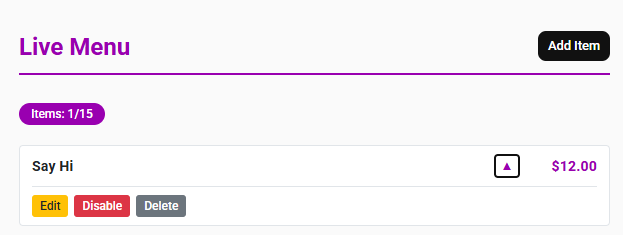
\includegraphics[width=\textwidth,height=0.2\textheight,keepaspectratio]{frontmatter/assets/Implementacao/liveMenu.png}
\caption{Menu de \textit{Items} - Criador}
\label{fig-menuCriador}
\end{figure}

As figuras~\ref{fig-menuViewer} e ~\ref{fig-menuCriador} representam as duas interfaces na aplicação.

\subsection{\textbf{Livestream}}

A criação do canal de \textit{streaming} é realizado pelo \gls{SDK} da AWS, esta operação devolve numa unica chamada, o \textbf{ARN do canal}, o \textbf{ingest endpoint} (servidor RTMP/RTMPS), o \textbf{playbackURL} (HLS para reprodução) e a \textbf{stream key}.~\ref{lst:liveStreamInfocreate}

\begin{lstlisting}[language=Java, caption={Criação do Canal - IVS}, label={lst:liveStreamInfocreate}]
        private async createLiveStreamInfo(account: Account): Promise<Result<LiveStreamInfo>> {
        
        const client = new IvsClient({
            region: process.env.AWS_REGION || 'eu-west-1',
                credentials: {
                    accessKeyId: process.env.AWS_ACCESS_KEY_ID,
                    secretAccessKey: process.env.AWS_SECRET_ACCESS_KEY,
                },
        });

        const input = {
            name: account.username.value,
            type: ChannelType.StandardChannelType,
            authorized: false
        };
        const command = new CreateChannelCommand(input);
        const response = await client.send(command);

        const liveStreamInfoOrError = LiveStreamInfo.create({
            accountId: account.accountId,
            channelArn: response.channel.arn,
            streamKey: response.streamKey.value,
            ingestEndpoint: response.channel.ingestEndpoint,
            playbackUrl: response.channel.playbackUrl,
        });

        return liveStreamInfoOrError;
    }
\end{lstlisting}

Na Listagem~\ref{lst:liveStreamInfodomain} a entidade \textit{LiveStreamInfo}, encapsula os artefactos retornados pelo AWS IVS com o \textit{accountId} do criador. O \textit{AggregateRoot}, valida a obrigatoriedade do \textit{accountId} e garante que a aplicação só consome um único agregado. 

\begin{lstlisting}[language=Java, caption={Classe de dominio - LiveStreamInfo}, label={lst:liveStreamInfodomain}]
interface LiveStreamInfoProps {
    channelArn: string;
    streamKey: string;
    ingestEndpoint: string;
    playbackUrl: string;
    accountId: AccountId;
}

export class LiveStreamInfo extends AggregateRoot<LiveStreamInfoProps> {
    get id(): UniqueEntityID {
        return this._id;
    }
    get livestreamInfoId(): LiveStreamInfoId {
        return LiveStreamInfoId.caller(this.id);
    }
    get channelArn(): string {
        return this.props.channelArn;
    }
    get streamKey(): string {
        return this.props.streamKey;
    }
    get ingestEndpoint(): string {
        return this.props.ingestEndpoint;
    }
    get playbackUrl(): string {
        return this.props.playbackUrl;
    }
    get accountId(): AccountId {
        return this.props.accountId;
    }
    set channelArn(channelArn: string) {
        this.props.channelArn = channelArn;
    }
    set streamKey(streamKey: string) {
        this.props.streamKey = streamKey;
    }
    
    set ingestEndpoint(ingestEndpoint: string) {
        this.props.ingestEndpoint = ingestEndpoint;
    }
    set playbackUrl(playbackUrl: string) {
        this.props.playbackUrl = playbackUrl;
    }

    private constructor(props: LiveStreamInfoProps, id?: UniqueEntityID) {
        super(props, id);
    }

    static create(props: LiveStreamInfoProps, id?: UniqueEntityID): Result<LiveStreamInfo> {
        const guarderProps= [
            { argument: props.accountId, argumentName: 'accountId' },
            { argument: props.channelArn, argumentName: 'channelArn' },
            { argument: props.streamKey, argumentName: 'streamKey' },
            { argument: props.ingestEndpoint, argumentName: 'ingestEndpoint' },
            { argument: props.playbackUrl, argumentName: 'playbackUrl' },
        ];
        const guardResult = Guard.againstNullOrUndefinedBulk(guarderProps);

        if (!guardResult.succeeded) {
            return Result.fail<LiveStreamInfo>(guardResult.message);
        }
        return Result.ok<LiveStreamInfo>(new LiveStreamInfo(props, id));
    }

}
\end{lstlisting}

A figura~\ref{fig-broadcastCriador} apresenta a interface de criador durante uma transmissão, e a listagem~\ref{lst:MediaStream}, liberta os recursos antigos, caso o criador escolha mudar de câmara, cria um objeto para pedir ao navegador tanto vídeo como áudio e guarda tanto os dispositivos como a câmara como o microfone.

\begin{figure}[H]
\centering
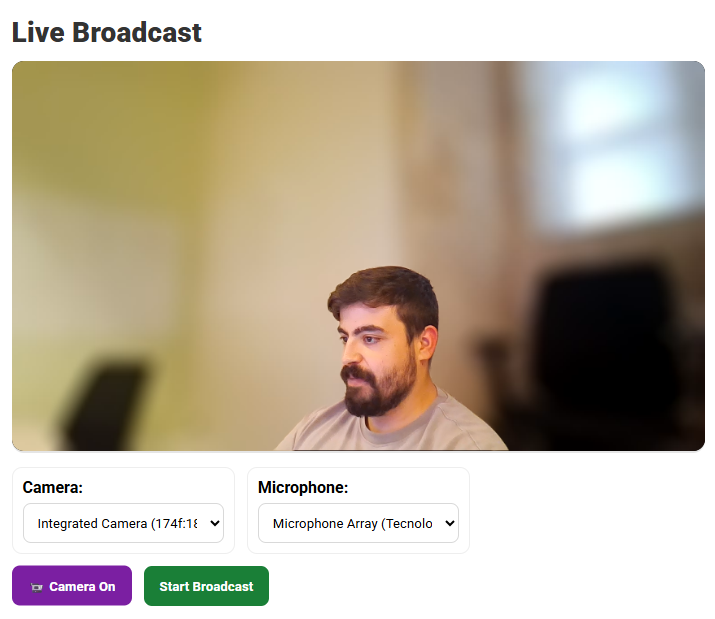
\includegraphics[width=\textwidth,height=0.4\textheight,keepaspectratio]{frontmatter/assets/Implementacao/broadcast.png}
\caption{Interface de Criador}
\label{fig-broadcastCriador}
\end{figure}

\begin{lstlisting}[language=Java, caption={Retirar a \textit{MediaStream} do navegador}, label={lst:MediaStream}]
const getMediaStream = async () => {
    try {
      if (mediaStreamRef.current) {
        mediaStreamRef.current.getTracks().forEach(track => track.stop());
        mediaStreamRef.current = null;
      }

      const constraints = {
        video: {
          deviceId: selectedVideoDevice ? { exact: selectedVideoDevice } : undefined,
          width: { ideal: 1920 },
          height: { ideal: 1080 }
        },
        audio: {
          deviceId: selectedAudioDevice ? { exact: selectedAudioDevice } : undefined
        }
      };

      const stream = await navigator.mediaDevices.getUserMedia(constraints);
      mediaStreamRef.current = stream;
      return stream;
    } catch (err) {
      setError("Error getting media stream: " + err.message);
      return null;
    }
  };
\end{lstlisting}


A figura~\ref{fig-broadcastCriadorViewer} apresenta a interface de visualizador durante uma transmissão, nela estão apresentados as configurações de utilizador como: \textit{play}, \textit{mute}, \textit{fullscreen} e uma definição para voltar ao instante em direto na transmissão.

Para renderizar o a transmissão foi usado o protocolo \gls{HLS} e a sua versão com menos latência (LL-HLS), o componente consome o \textit{URL} de \textit{playback} e recebe informação diretamente da AWS.

\begin{figure}[H]
\centering
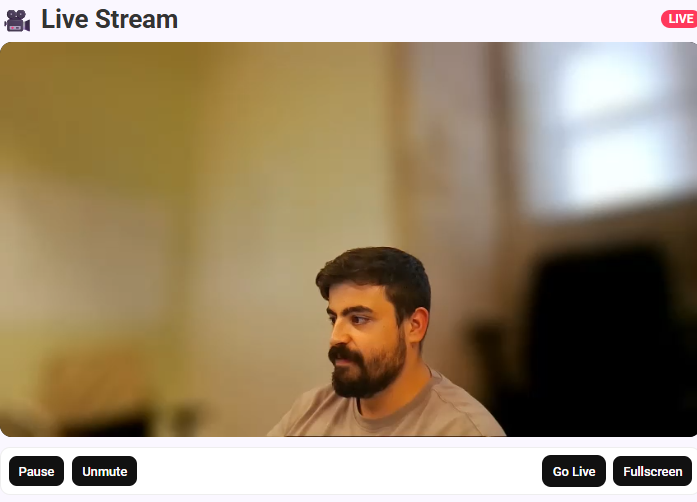
\includegraphics[width=\textwidth,height=0.4\textheight,keepaspectratio]{frontmatter/assets/Implementacao/viewer.png}
\caption{Interface de Utilizador}
\label{fig-broadcastCriadorViewer}
\end{figure}


\section{Testes} 

Nesta secção, são apresentadas evidências de testes tanto de domínio como \textit{end-2-end}.

\subsubsection{Testes de Domínio}

\begin{itemize}
  \item \textbf{LiveMenu}
    \begin{itemize}
      \item Cria-se um \textit{LiveMenu} válido.
      \item Falha quando \texttt{accountId} está ausente.
    \end{itemize}

  \item \textbf{LiveMenuItem}
    \begin{itemize}
      \item Cria-se um \textit{LiveMenuItem} válido.
      \item Falha quando \texttt{name} está ausente.
      \item Falha quando \texttt{price} está ausente.
      \item Falha quando \texttt{liveMenuId} está ausente.
      \item Falha quando \texttt{name} está vazio.
      \item Falha quando \texttt{name} excede o comprimento permitido.
      \item Falha quando \texttt{price} é negativo.
    \end{itemize}

  \item \textbf{LiveStream}
    \begin{itemize}
      \item Cria-se um \textit{LiveStream} válido.
      \item Falha quando \texttt{startTime} está ausente.
      \item Falha quando \texttt{livestreamInfo} está ausente.
    \end{itemize}

  \item \textbf{LiveStreamInfo}
    \begin{itemize}
      \item Cria-se um \textit{LiveStreamInfo} válido.
      \item Falha quando \texttt{accountId} está ausente.
      \item Falha quando \texttt{channelArn} está ausente.
      \item Falha quando \texttt{streamKey} está ausente.
      \item Falha quando \texttt{ingestEndpoint} está ausente.
      \item Falha quando \texttt{playbackUrl} está ausente.
    \end{itemize}

  \item \textbf{Tier}
    \begin{itemize}
      \item Cria-se um \textit{Tier} válido.
      \item Falha quando \texttt{perks} está vazio.
      \item Falha quando \texttt{name} está ausente.
      \item Falha quando \texttt{colorCode} está ausente.
      \item Falha quando \texttt{price} está ausente.
    \end{itemize}
\end{itemize}

Na Figura~\ref{fig-domainTests}, são apresentados os resultados dos testes.

\begin{figure}[H]
\centering
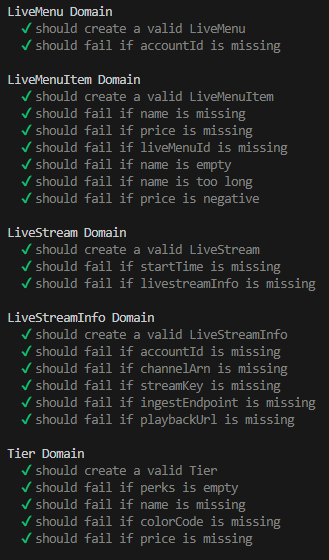
\includegraphics[width=\textwidth,height=0.4\textheight,keepaspectratio]{frontmatter/assets/design/tests.png}
\caption{Testes de Domínio}
\label{fig-domainTests}
\end{figure}

Para realizar os testes de domínio usaram-se algumas bibliotecas do \textbf{NPM} como \textbf{Jest}, \textbf{Mocha} e \textbf{Chai}.

\begin{lstlisting}[language=Java, caption={Teste de criação do LiveStreamInfo}, label={lst:liveStreamInfoTest}]
    it("should create a valid LiveStreamInfo", () => {
        const props = {
            accountId,
            channelArn: "arn:aws:ivs:channel",
            streamKey: "key123",
            ingestEndpoint: "endpoint",
            playbackUrl: "url"
        };
        const result = LiveStreamInfo.create(props);
        expect(result.isSuccess).to.equal(true);
        expect(result.getValue().accountId).to.equal(accountId);
        expect(result.getValue().channelArn).to.equal("arn:aws:ivs:channel");
        expect(result.getValue().streamKey).to.equal("key123");
        expect(result.getValue().ingestEndpoint).to.equal("endpoint");
        expect(result.getValue().playbackUrl).to.equal("url");
    });
\end{lstlisting}

Neste teste, os \textit{props} são construidos com todos os atributos necessários. De seguida, invoca-se o método \textit{create} da classe \textit{LiveStreamInfo}, que valida se os atributos foram bem definidos.
Por fim, o teste passa de o método \textbf{create} devolver uma entidade igual ao respetivo valor fornecido pelos \textit{props}.


\subsubsection{Testes \textit{end-2-end}}

O principal objetivo destes testes é garantir que uma transmissão pode ser iniciada e parada de forma consistente, incluindo ciclos rápidos e proteção contra dois cliques. Também é importante capturar os estados da interface de utilizador, e manter moderar o \textit{low latency chat}.

\textbf{Livestream Tests}
    \begin{itemize}
      \item Começar e parar a transmissão.
      \item Vários ciclos de começo e termino de transmissão.
      \item Prevenir cliques duplos.
    \end{itemize}
    
\textbf{Low Latency Chat Tests}
    \begin{itemize}
      \item Enviar mensagem normal. 
      \item Tamanho mínimo da mensagem.
      \item Tamanho máximo da mensagem.
      \item Envio de \textit{emojis}.
      \item Validação da pontuação (acentos).
      \item Validação de caracteres especiais.
    \end{itemize}

Os seguintes excertos de código demonstram a configuração do ambiente \textit{end-2-end}. A lista~\ref{lst:criaçãoDoAmbientedeTestes} parametriza o contexto do \textit{browser} com as permissões e os dispositivos. A lista~\ref{lst:beforeEach} e a lista~\ref{lst:livestreamstartstoptest} organizam o ambiente de testes, realizam a autenticação, navegação para a página de transmissão, as operações de iniciar e parar a transmissão. Por fim, a lista~\ref{lst:livestreame2etest} mostra o código literal do teste.


\begin{lstlisting}[language=Java, caption={Criação do ambiente de testes}, label={lst:criaçãoDoAmbientedeTestes}]
 
 test.use({
  browserName: 'chromium',
  channel: 'chrome',
  permissions: ['camera', 'microphone'],
  launchOptions: {
    args: [
      '--use-fake-ui-for-media-stream',
      '--use-fake-device-for-media-stream',
      '--no-sandbox',
    ],
  },
});

\end{lstlisting}

\begin{lstlisting}[language=Java, caption={Configuração do ambiente de testes}, label={lst:beforeEach}]

test.describe('Private Stream Tests (refactored)', () => {
  test.beforeEach(async ({ page }) => {
    const auth = new Auth(page);        
    const profile = new Profile(page); 

    await auth.openHome('https://dev.onlyyestest.com/'); 
    await auth.openSignIn();
    await auth.fillEmailAndPassword(email, password);
    await auth.submitSignIn(); 

    await profile.openSettings();
    const stream = new Stream(page);   
    await stream.openPrivateLive();     
  });

\end{lstlisting}

\begin{lstlisting}[language=Java, caption={Operações de inicio e fim de transmissão}, label={lst:livestreamstartstoptest}]

class Stream {
  private readonly btnStart;
  private readonly btnStop;

  constructor(private readonly page: Page) {
    this.btnStart = page.getByRole('button', { name: 'Start Broadcast' });
    this.btnStop  = page.getByRole('button', { name: 'Stop Broadcast' });
  }

  async start(): Promise<void> {
    await this.expectStartVisible();
    await this.btnStart.click();
    await this.expectStopVisible();
  }

  async stop(): Promise<void> {
    await this.expectStopVisible();
    await this.btnStop.click();
    await this.expectStartVisible();
  }

  async expectStartVisible(): Promise<void> {
    await expect(this.btnStart).toBeVisible({ timeout: 8000 });
  }
  async expectStopVisible(): Promise<void> {
    await expect(this.btnStop).toBeVisible({ timeout: 5000 });
  }
}
\end{lstlisting}

\begin{lstlisting}[language=Java, caption={Teste de inicio e fim de transmissão}, label={lst:livestreame2etest}]

  test('Start and stop broadcast stream', async ({ page }) => {
    const stream = new Stream(page);
    await stream.start();
    await stream.stop();
  });
});

\end{lstlisting}

\section{Avaliação da solução} 

Na empresa, foram testados alguns \textit{endpoints} para verificar o comportamento da solução na infraestrutura AWS. Na imagem~\ref{img:testeCarga}, mostra um teste de carga realizado num dos destes \textit{endpoints}. Conseguimos observar que em média, a resposta dos pedidos é 200 milissegundos, o que para a empresa foi satisfatório. 


\begin{figure}[H]
\centering
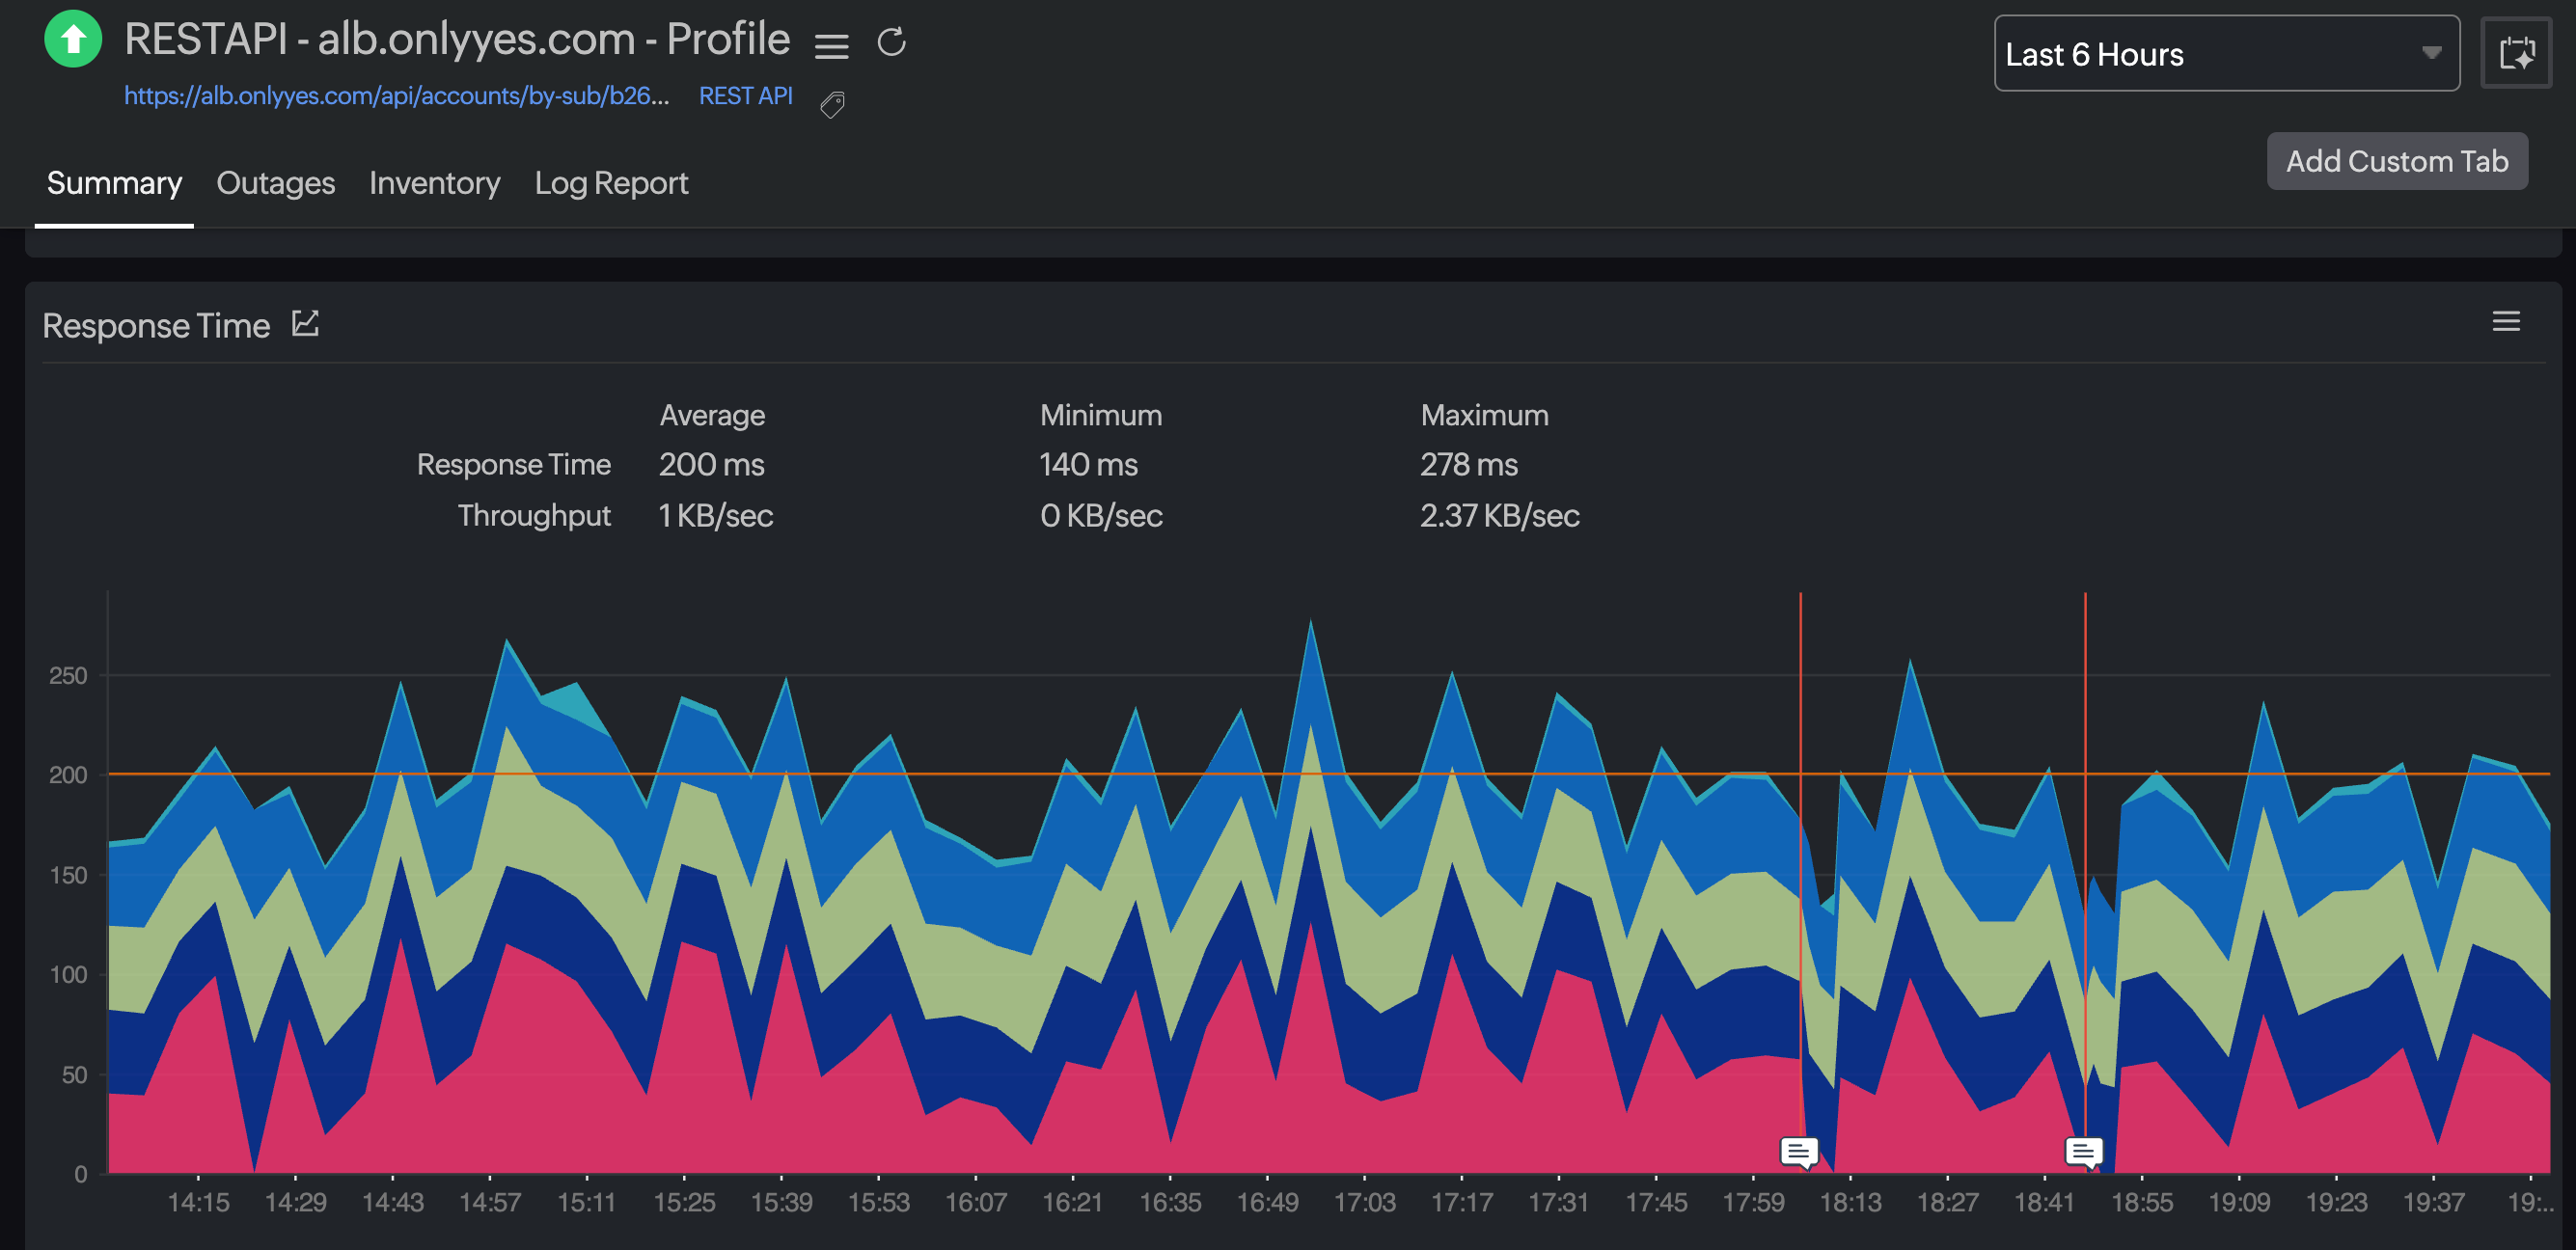
\includegraphics[width=\textwidth,height=0.4\textheight,keepaspectratio]{frontmatter/assets/Implementacao/image (1).png}
\caption{Teste de Carga}
\label{fig-domainTests}
\end{figure}